\label{sec:Introduction}
\begin{figure*}
	\centering
		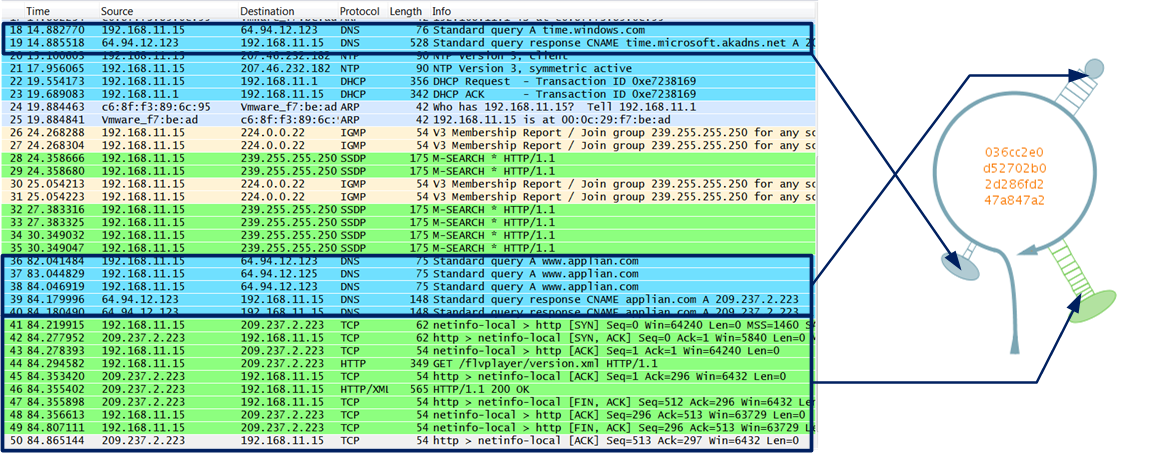
\includegraphics[width=0.78\linewidth]{pics/Mapping.png}
	\label{fig:Mapping}
        \caption{We illustrate our mapping scheme with a simple network packet
        traces generated by malware~(036cc2e0): there are three
        streams of packets~(as highlighted by rectangles in the flow records
        produced by Wireshark~\cite{Wireshark}) are mapped to three cilia in
        the cell view on the right. The user can select a cilium for detailed
        information about the stream.}
\end{figure*}


Malware remains at the forefront of most security threats on the Internet. Nearly every existing malware instance relies on network communication to facilitate its attacks, such as communicating with its command and control (C\&C) server, sending spam emails or operating in a fast-flux service network. Therefore, network traces are commonly used to characterize a malware sample's behavior. As an essential technology that combats illegal income for the attackers, malware analysis has been playing a crucial role in supplying signatures for detection systems.

There is a growing need for visual presentations in the workplace of malware analysis: new instances of ``in the wild'' malware samples are collected daily. In a typical analysis scenario, each malware instance is run in a controlled environment where its host-level and network-level activities are captured as host and network traces. In order to keep track of each sample, security researchers maintain large databases of network traces. Due to their sheer size, it is a daunting task to look into the details of each sample.

Current malware analysis approaches pose several challenges to the analytic
process itself which complicate visualization design. First, network traces
often contain network information that is not relevant to the actual malicious
behavior. For example, network traffic generated by the operating system.
Having to visualize everything not only complicates the design, but also causes
confusion to the analysts. Malware samples seen in the wild tend to use only a
couple of protocols, such as DNS and TCP, to perform their malicious behavior.
To reduce clutter, we do not visualize less common protocols by default.
Second, the analyst can easily lose the big picture of malware activities by
focusing on individual packets. To handle this, we aggregate packets into
streams separated by protocol. Specifically, we focus on DNS and TCP streams as
they are often used by malware for communication. Third, streams can vary
drastically in packet size and these uneven distributions present themselves in
nearly every attribute space (e.g. total size of transmission, starting time,
duration). Linearly mapping these attributes not only consumes screen
real-estate, but also draws the viewer's attention away from those small but
potentially important streams. Lastly, showing all relevant attributes in a
single, clear view requires an original design. In the absence of an intuitive
presentation of sets of network traces, malware behavior analysis will remain
tedious.

The goal of this paper is to present a visualization system and a model design
that address the above challenges. Our work claims the following contributions:
\begin{itemize}

	\item \textbf{Data collection and preprocessing.} The malware network traces were captured by packet sniffer software in a controlled environment. The preprocessing consists of two steps: \emph{pruning} and \emph{bundling}. The raw network data are pruned by preserving protocols known to be used commonly by malware seen in the wild be default. Other protocols can be viewed if an analyst wishes to do so. Then we bundle the packets according to their protocols and hosts so that each stream of communication is semantically clear.

	\item \textbf{Interface and visualization metaphor.} We design an intuitive view, the \emph{cell view}, to represent a set of streams generated by any malware instance. A cell view consists of a \emph{circular timeline}, a \emph{disk panel} to display details-on-demand, and a set of \emph{cilia} oriented clockwise along the timeline to represent the set of streams. This metaphorical structure allows the viewer to select and compare among streams as well as between malware instances.

	\item \textbf{Mapping and layout techniques for sparsely distributed attributes.} As explained earlier, the majority of the communication~(in terms of the number of packets, transmission size) takes place within a small percentage of streams. Also, many streams may occur within a short period of time. To cope with these uneven distributions, we use geometric sequences and inverse logarithms to map discrete or continuous attribute values. We also present a recursive angle mapping algorithm that helps produce equalized layout for viewing streams that are cluttered over time.
\end{itemize}

This paper is organized as follows. Section~\ref{sec:prior} introduces several related security visualization systems. Section~\ref{sec:overview} presents an expository account of malware analysis infrastructure for the benefit of readers who are not familiar with the technique. We then introduce our design and implementation in Section\ref{sec:implementation}. We apply the visualization model to a corpus of real-world malware samples and Section~\ref{sec:interaction} introduces user interaction scenarios with different components of MalwareVis. Finally, Section~\ref{sec:discuss} discusses and reflects on the project process; Section~\ref{sec:conclude} concludes the paper.




